% abtex2-modelo-artigo.tex, v-1.9.2 laurocesar
% Copyright 2012-2014 by abnTeX2 group at http://abntex2.googlecode.com/ 
%

% ------------------------------------------------------------------------
% ------------------------------------------------------------------------
% abnTeX2: Modelo de Artigo Acadêmico em conformidade com
% ABNT NBR 6022:2003: Informação e documentação - Artigo em publicação 
% periódica científica impressa - Apresentação
% ------------------------------------------------------------------------
% ------------------------------------------------------------------------

\documentclass[
	% -- opções da classe memoir --
	article,			% indica que é um artigo acadêmico
	11pt,				% tamanho da fonte
	oneside,			% para impressão apenas no verso. Oposto a twoside
	a4paper,			% tamanho do papel. 
	% -- opções da classe abntex2 --
	%chapter=TITLE,		% títulos de capítulos convertidos em letras maiúsculas
	%section=TITLE,		% títulos de seções convertidos em letras maiúsculas
	%subsection=TITLE,	% títulos de subseções convertidos em letras maiúsculas
	%subsubsection=TITLE % títulos de subsubseções convertidos em letras maiúsculas
	% -- opções do pacote babel --
	english,			% idioma adicional para hifenização
	brazil,				% o último idioma é o principal do documento
	sumario=tradicional
	]{abntex2}


\ifthenelse{\equal{\ABNTEXisarticle}{true}}{%
\renewcommand{\maketitlehookb}{}
}{}

% ---
% PACOTES
% ---

% ---
% Pacotes fundamentais 
% ---

\usepackage{lmodern}			% Usa a fonte Latin Modern
\usepackage[T1]{fontenc}		% Selecao de codigos de fonte.
\usepackage[utf8]{inputenc}		% Codificacao do documento (conversão automática dos acentos)
\usepackage{indentfirst}		% Indenta o primeiro parágrafo de cada seção.
\usepackage{nomencl} 			% Lista de simbolos
\usepackage{color}				% Controle das cores
\usepackage{graphicx}			% Inclusão de gráficos
\usepackage{microtype} 			% para melhorias de justificação
\usepackage{subcaption}
\let\newfloat\undefined
\usepackage[capposition=top]{floatrow}
%\usepackage{amsmath}
\usepackage{scalerel,mathtools}
\usepackage{multirow}
\usepackage[table,xcdraw]{xcolor}
\usepackage{listings}

% ---
\DeclareMathOperator*{\varsum}{\scalerel*{\scriptstyle\Sigma}{\sum}}
% ---
% Pacotes adicionais, usados apenas no âmbito do Modelo Canônico do abnteX2
% ---
\usepackage{lipsum}				% para geração de dummy text
% ---
		
% ---
% Pacotes de citações
% ---
\usepackage[brazilian,hyperpageref]{backref}	 % Paginas com as citações na bibl
\usepackage[alf]{abntex2cite}	% Citações padrão ABNT
% ---


% ---
% Configurações do pacote backref
% Usado sem a opção hyperpageref de backref
\renewcommand{\backrefpagesname}{Citado na(s) página(s):~}
% Texto padrão antes do número das páginas
\renewcommand{\backref}{}
% Define os textos da citação
\renewcommand*{\backrefalt}[4]{
	\ifcase #1 %
		Nenhuma citação no texto.%
	\or
		Citado na página #2.%
	\else 
		Citado #1 vezes nas páginas #2.%
	\fi}%
% ---

% --- Informações de dados para CAPA e FOLHA DE ROSTO ---
\titulo{Lógica, Apenas Lógica}
\tituloestrangeiro{Logic, Logic Only}

\autor{
Renan Aparecido Stuchi\thanks{E-mail: \href{malito:ren.stuchi@gmail.com}{ren.stuchi@gmail.com} | GitHub: \url{https://github.com/RenStu/logic} } }

\local{Brasil}
\data{2020, v-1.1.0}
% ---

% ---
% Configurações de aparência do PDF final

% alterando o aspecto da cor azul
\definecolor{blue}{RGB}{41,5,195}

% informações do PDF
\makeatletter
\hypersetup{
     	%pagebackref=true,
		pdftitle={\@title}, 
		pdfauthor={\@author},
    	pdfsubject={Filosofia lógica e metafísica},
	    pdfcreator={LaTeX with abnTeX2},
		pdfkeywords={lógica. }{nada. }{tudo. }{binômio. }{binomial de expansão. }{teorema central do limite. }{consciência. }{infinito. }{tempo. }{espaço. }{gravidade. }{matéria escura. }{energia escura. }{antimatéria. }{buraco negro.},
%		pdfkeywords={lógica. }{nada. }{tudo. }{infinito. },
		colorlinks=true,       		% false: boxed links; true: colored links
    	linkcolor=blue,          	% color of internal links
    	citecolor=blue,        		% color of links to bibliography
    	filecolor=magenta,      	% color of file links
		urlcolor=blue,
		bookmarksdepth=4
}
\makeatother
% --- 

% ---
% compila o indice
% ---
\makeindex
% ---

% ---
% Altera as margens padrões
% ---
\setlrmarginsandblock{3cm}{3cm}{*}
\setulmarginsandblock{3cm}{3cm}{*}
\checkandfixthelayout
% ---

% --- 
% Espaçamentos entre linhas e parágrafos 
% --- 

% O tamanho do parágrafo é dado por:
\setlength{\parindent}{1.3cm}

% Controle do espaçamento entre um parágrafo e outro:
\setlength{\parskip}{0.2cm}  % tente também \onelineskip

% Espaçamento simples
\SingleSpacing

% Fomatação C# code
%\setmonofont{Consolas} %to be used with XeLaTeX or LuaLaTeX
\definecolor{bluekeywords}{rgb}{0,0,1}
\definecolor{greencomments}{rgb}{0,0.5,0}
\definecolor{redstrings}{rgb}{0.64,0.08,0.08}
\definecolor{xmlcomments}{rgb}{0.5,0.5,0.5}
\definecolor{types}{rgb}{0.17,0.57,0.68}
\lstset{language=[Sharp]C,
	captionpos=b,
	%numbers=left, %Nummerierung
	%numberstyle=\tiny, % kleine Zeilennummern
	frame=lines, % Oberhalb und unterhalb des Listings ist eine Linie
	showspaces=false,
	showtabs=false,
	breaklines=true,
	showstringspaces=false,
	breakatwhitespace=true,
	escapeinside={(*@}{@*)},
	commentstyle=\color{greencomments},
	morekeywords={partial, var, value, get, set},
	keywordstyle=\color{bluekeywords},
	stringstyle=\color{redstrings},
	basicstyle=\ttfamily\tiny,
}


% ----
% Início do documento
% ----
\DeclareUnicodeCharacter{2212}{-}
\begin{document}

	\pagestyle{plain}
	
	% Seleciona o idioma do documento (conforme pacotes do babel)
	%\selectlanguage{english}
	\selectlanguage{brazil}


	% Retira espaço extra obsoleto entre as frases.
	\frenchspacing 

	% ----------------------------------------------------------
	% ELEMENTOS PRÉ-TEXTUAIS
	% ----------------------------------------------------------
		% Resumo
		% ----------------------------------------------------------
% ELEMENTOS PRÉ-TEXTUAIS
% ----------------------------------------------------------
% página de titulo
\vspace{-15mm}
\maketitle
\vspace{-8mm}
% resumo em português
\begin{resumoumacoluna}
\vspace{-2mm}
	Neste artigo pretende-se introduzir uma teoria a respeito da origem de tudo. O objetivo inicial é responder se existe algo ao invés de nada. Essa pergunta vem incomodando a filosofia e a ciência até os dias de hoje. A resposta a essa pergunta está na compreensão de que a lógica em sua essência remete ao nada, que NÃO É, ou seja, nega a si mesmo (nega ser). A negação de si gera expansões binomiais, no qual suas amostras combinadas em cada passo dessa expansão se aproximam da distribuição normal e se aproximam do centro dessa distribuição infinitamente, o que configura o teorema central do limite. Os passos da expansão binomial regidos pela probabilidade descrita no teorema central do limite compreendem a consciência e tornam visíveis o que é e o porquê de seus aspectos mais perceptíveis: infinito, tempo, espaço, gravidade, matéria escura, energia escura, antimatéria e buraco negro. Como essência da expansão binomial, do teorema central do limite e da consciência e seus aspectos tem-se a lógica em sua dualidade, que por um lado NÃO É e por outro É ilógica, imutável e inexistente, uma vez que a existência está em tudo aquilo que NÃO É. 
 \vspace{\onelineskip} 
 \noindent
 
 \textbf{Palavras-chaves}: lógica. nada. tudo. binômio. expansão binomial. teorema central do limite. consciência. infinito. ondas. tempo. espaço. forças fundamentais. gravidade. matéria escura. energia escura. antimatéria. buraco negro.
\end{resumoumacoluna}

% resumo em inglês
\renewcommand{\resumoname}{Abstract}
\begin{resumoumacoluna}
 \begin{otherlanguage*}{english}
\vspace{-2mm}
	This article aims to introduce the theory about the origin of everything. The initial goal is to answer if there is something instead of nothing. This question has been bothering philosophy and science to this day. The answer to this question lies in understanding that logic in its essence refers to nothing, which IS NOT, that is, denies itself (denies being). Self-denial generates binomial expansions, in which their combined samples at each step of this expansion approach the normal distribution and approach the center of this distribution infinitely, which configures the central limit theorem. The steps of binomial expansion governed by the probability described in the central limit theorem comprise consciousness and make visible what it is and why its most noticeable aspects are: infinity, time, space, gravity, dark matter, dark energy, antimatter and black hole. The essence of binomial expansion, the central limit theorem and consciousness and its aspects is logic in its duality, which on the one hand IS NOT and on the other hand IS illogical, unchanging and non-existent, since existence is in all that IS NOT.
	\vspace{\onelineskip} 
	\noindent
	
	\textbf{Keywords}: logic. nothing. all. binomial. binomial expansion. central limit theorem. consciousness. infinite. waves. time. space. fundamental forces. gravity. dark matter. dark energy. antimatter. black hole.
 \end{otherlanguage*}  
\end{resumoumacoluna}

%\begin{center}\smaller
%\textbf{Identificação e disponibilidade}: elemento opcional. Pode ser indicado 
%o endereço eletrônico, DOI, suportes e outras informações relativas ao acesso.
%\end{center}

	% ----------------------------------------------------------
	% ELEMENTOS TEXTUAIS
	% ----------------------------------------------------------
		% Introdução
		% ----------------------------------------------------------
% Introdução
% ----------------------------------------------------------
\section*{Introdução}
\addcontentsline{toc}{section}{Introdução}

O raciocínio deste texto surgiu como resposta a pergunta mais essencial que a filosofia pode formular e que a ciência até então não foi capaz de responder plenamente, que é se existe algo ao invés de nada ou porque existe algo ao invés de nada? 
Essa pergunta foi feita pela primeira vez pelo filosofo Gottfried Wilhelm Leibniz em uma carta de 1697 e é frequentemente descrita como a maior questão filosófica \cite{ leibnizbrasil_origem_das_coisas}.

A resposta a essa pergunta vem da resposta do que é a lógica. Ao explorar o que a lógica é e o que ela NÃO É, deu origem a uma teoria a respeito da origem de tudo, de todas as coisas. A lógica em sua essência remete ao nada, que NÃO É, ou seja, nega a si (nega ser). A negação de si gera expansões binomiais, no qual suas amostras combinadas em cada passo dessa expansão se aproximam da distribuição normal e se aproximam do centro dessa distribuição infinitamente, o que configura o teorema central do limite. A compreensão destes dois conceitos matemáticos, expansão binomial e teorema central do limite, são essenciais para entendimento dessa teoria.

Os passos da expansão binomial, originados da negação lógica a si, regidos pela probabilidade descrita no teorema central do limite compreendem a consciência e tornam visíveis o que é e o porquê de seus aspectos mais perceptíveis: infinito, tempo, espaço, gravidade, matéria escura, energia escura e buraco negro. Ao responder a pergunta essencial deste estudo também é possível responder as principais questões da ciência, o que é e o porquê é a consciência e seus aspectos, pois são provenientes de um mesmo aspecto lógico.

A lógica NÃO SER é consonante com o NADA, pois se a lógica NÃO É ela também É seu contrário, ou seja, ilógica e imutável. Nessa dualidade, tem-se a existência fundamentada pela lógica que "nega a si", enquanto, por outro lado É ilógica, imutável e inexistente. O texto está disposto na seguinte hierarquia:
{\small
\begin{enumerate}[label*=\arabic*.]
   \item Lógica
   \begin{enumerate}[label*=\arabic*.]
	   \item Expansão binomial
	   \item Teorema central do limite
	   \item Consciência
		   \begin{enumerate}[label*=\arabic*.]
			   \item Infinito
			   \item Tempo
			   \item Espaço
			   \item Gravidade
			   \item Matéria escura e energia escura
			   \item Antimatéria
			   \item Buraco negro
			   \item Coexistência inferida
			   \item Foco
		   \end{enumerate}   
   \end{enumerate}
\end{enumerate}
}
%\bigbreak
Primeiro é definido o que é a lógica e principalmente o que ela NÃO É, assim é apresentado sua consonância ao nada. Depois é descrito como essa lógica primordial, essência de qualquer lógica, se desenvolve gerando novas lógicas por meio de sua expansão binomial. Em seguida é observado que as amostras combinadas em cada passo dessa expansão são regidas pela probabilidade descrita no teorema central do limite o qual da origem ao que a consciência. A negação da nada a si gera as expansões binomiais que são regidas pela probabilidade descrita no teorema central do limite (consciência) é o aspecto lógico responsável em dizer o porquê e o que é o infinito, o tempo, o espaço, a gravidade, a matéria escura, a energia escura e o buraco negro, inicialmente. 
		
		% Lógica - conteúdo
		% ----------------------------------------------------------
% Seção Lógica - Principal
% ----------------------------------------------------------
\section{Lógica}
Segundo o dicionário online de Português Dicio\cite{dicio_logica}, a palavra lógica se refere a:
\begin{enumerate}
   \item Modo de raciocinar coerente que \underline{expressa uma relação de causa e consequência};
   \item Maneira coerente através da qual os \underline{fatos ou situações se encadeiam}. 
\end{enumerate}
 
\bigbreak
A palavra lógica expressa uma relação de causa e consequência ou fatos encadeados. Pode-se distinguir como essência dessas duas definições o movimento, a mudança, a transição. A palavra lógica, em sua essência, se encaixa perfeitamente na definição do NADA − NÃO SER.  A lógica NÃO SER é consonante com o NADA, pois se a lógica NÃO É ela também É seu contrário, ou seja, ilógica e imutável. Nessa dualidade, tem-se a existência fundamentada pela lógica que "nega a si", enquanto, por outro lado É ilógica, imutável e inexistente. A expressão "negação de si" refere-se à negação do SER - NÃO SER. 

A lógica está centrada na mudança e a mudança está centrada naquilo que NÃO É, uma vez que aquilo que É não pode deixar de SER. A mudança demanda que, em algum momento, algo DEIXE DE SER o que fora a se transformar. Em \citeonline{brasilescola_parmenides}, Parmênides  o filósofo da unidade e da identidade do SER, diz que a contínua mudança é a principal característica do não ser. Para Parmênides o SER é uno, eterno, não gerado e imutável.

A lógica SER ilógica não a impede de NÃO SER.  Na dualidade SER e NÃO SER, o SER limita e define o NÃO SER \textit{ad infinitum}. É possível se aproximar da definição do SER enumerando e definindo infinitamente tudo o que ele NÃO É.

\begin{figure}[H]
\caption{Analogia da lógica primordial}
\label{fig:primordial_logic_representation}
\centering
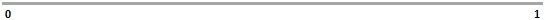
\includegraphics[scale=1]{sections/images/primordial_logic_representation.jpg}
\floatfoot{Reta utilizada para representar e validar o conceito da lógica primordial.}%\footnotemark}
\end{figure}
%\footnotetext{Fonte: note}

Com base na Figura \ref{fig:primordial_logic_representation} pode-se extrair as seguintes observações em relação aos pontos \textbf{0}, \textbf{1} e o \textbf{intervalo} entre eles:
\begin{description}
   \item[Ponto 1 - {[1,1]}] É ilógico, pois é a totalidade não fracionada da reta.
   \item[Ponto 0 - {[0,0]}] É ilógico, pois é um ponto nulo incapaz de negar a si, dado que toda lógica ou sublógica (fração lógica) deve se manter negado a si, uma que essa é a premissa básica da lógica. A lógica NÃO É em sua essência, primordialmente.
   \item[Intervalo - $\textbf{{[0,1[ x ]0,1]}}$] A lógica é possível apenas na representação das frações ou intervalos dos pontos \textbf{0} e \textbf{1}. Uma fração da reta nega ser a reta, pois é apenas uma parte dela. Os subintervalos são hábeis a negar a si infinitamente, garantindo a premissa primordial da lógica e suas sublógicas, negar a si. 
\end{description}

\begin{figure}[H]
\caption{Primeiro momento lógico}
\label{fig:first_logical_moment}
\centering
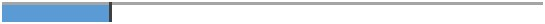
\includegraphics[scale=1]{sections/images/first_logical_moment.jpg}
\floatfoot{Reta fracionada em dois intervalos representando o primeiro momento lógico.}%\footnotemark}
\end{figure}
%\footnotetext{Fonte: note}

Na Figura \ref{fig:first_logical_moment} a união do traço à reta é a representação de uma divisão lógica, pois é da negação da lógica em SER que surgi esses dois intervalos lógicos ou duas sub-lógicas. O segmento em azul representa a negação da lógica em SER o todo ilógico nesse primeiro momento. As duas frações geradas pela negação lógica negam SER a reta, pois são apenas intervalos delas e são capazes de negar a si infinitamente, garantindo a premissa primordial da lógica NÃO SER. 

% ----------------------------------------------------------
% Subseção Expansão binomial
% ----------------------------------------------------------
\subsection{Expansão binomial}
A lógica primordial (negação de si) cria expansões binomiais infinitas. O primeiro momento lógico é o início de uma dessas expansões, porém existem infinitas possibilidades de negação do primeiro momento lógico, o que revela as infinitas expansões binomiais. Uma expansão binomial é análoga a um universo. É importante observar que o primeiro momento lógico negar SER ilógico não transforma o ilógico em lógico, negar não é transformar. É essa dualidade da lógica (SER ilógica e NÃO SER lógica) que garante as infinitas expansões binomiais, uma vez que o ilógico é imutável e por isso pode ser negado infinitamente.

\begin{quote}
"Em nossos dias vemos a expansão binomial de uma forma limpa e prática, sendo considerada um dos desenvolvimentos mais lindos e elegantes da matemática, vista com simplicidade em todos os níveis de ensino e pesquisa." \cite{ufpr_binomio_newton}.
\end{quote}
\begin{align*}
(x+a)^n &= \sum_{p=0}^{n}\binom{n}{p} a^p x^{n-p}
\end{align*}

\begin{figure}[H]
\caption{Momentos lógicos iniciais}
\label{fig:third_logical_moment}
\centering
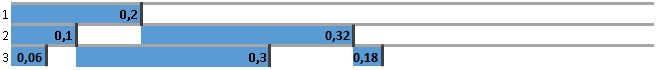
\includegraphics[scale=.85]{sections/images/third_logical_moment.jpg}
\floatfoot{Exemplo dos três primeiros momentos de uma expansão.}%\footnotemark}
\end{figure}
%\footnotetext{Fonte: note}

Com base na Figura \ref{fig:third_logical_moment} pode-se extrair as seguintes observações em relação ao primeiro, segundo e terceiro momentos lógicos:
\begin{description}
   \item[Primeiro momento lógico] A negação da lógica primordial a si, a subdivide em duas unidades, que somadas são o todo ilógico. Apesar dessas partes terem proporções diferentes, elas exprimem as mesmas quantidades de pontos ou possibilidades de mudança, uma vez que são representações da lógica primordial, que ad infinitum. A parte fracionada em azul representa a proporção da negação lógica em relação à sua unidade.
   \item[Segundo momento lógico] É gerado pela negação das duas sub-lógicas primordiais, fracionadas no primeiro momento lógico. Na impossibilidade dessas frações lógicas do primeiro momento lógico continuar negando a si, faria com que elas fossem incapazes de negar suas unidades que formam o todo, ou seja, seriam incapazes de negar as duas unidades e por consequência o todo que é formado precisamente por elas, o que faria da lógica apenas ilógica, uma unicidade. As partes fracionadas em azul representam a proporção da negação lógica em relação à sua respectiva unidade.
   \item[Terceiro momento lógico] Decorre da negação do segundo momento lógico, assim como o segundo momento lógico decorre da negação do primeiro e assim por diante.
\end{description}

A cada negação ou subnegação da lógica primordial, seus novos valores são influenciados pelos valores adjacentes do momento lógico anterior. Na figura \ref{fig:imposition_of_binomial_expansion}, a lógica primordial nega a si gerando o primeiro momento lógico com o valor [0,2].  No segundo momento lógico, suas subdivisões estão contidas no limite imposto pelo valor do primeiro momento lógico. Os pontos do terceiro momento lógico, por exemplo, sofrem as imposições dos valores do segundo momento lógico que por sua vez sofrem a imposição do primeiro. Os valores de momentos lógicos descendentes sofrem imposições acumulativas dos valores dos momentos lógicos anteriores. À imposição de um valor em seus dois valores imediatamente descendentes denominou-se sincronismo lógico. Isso é o que pode ser visto no triângulo de pascal.

\begin{figure}[H]
\caption{Imposição da expansão binomial}
\label{fig:imposition_of_binomial_expansion}
\centering
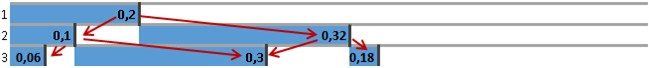
\includegraphics[scale=.85]{sections/images/imposition_of_binomial_expansion.jpg}
\floatfoot{Imposição acumulativa aos momentos lógicos descendentes.}%\footnotemark}
\end{figure}
%\footnotetext{Fonte: note}

No triângulo de pascal, Figura \ref{fig:pascal_triangle}, cada número é os dois números acima mais próximos somados. Esse número representa quantos diferentes possíveis caminhos levam até ele. Por exemplo, o número [4], na Figura \ref{fig:pascal_triangle}, representa os quatro diferentes caminhos que levam até ele. Um outro aspecto interessante do triângulo de pascal é a sequência de Fibonacci, Figura \ref{fig:pascal_triangle_fibonacci} \cite{mathisfun_pascal_triangle}.  

\begin{figure}[H]
\centering
	\begin{subfigure}[H]{0.47\linewidth}
	\centering
	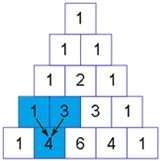
\includegraphics[width=.55\linewidth]{sections/images/pascal_triangle.jpg}
	\caption{}
	\label{fig:pascal_triangle}
	\end{subfigure}
\hfill
	\begin{subfigure}[H]{0.47\linewidth}
	\centering
	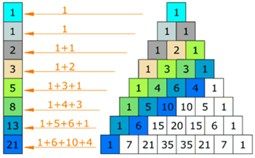
\includegraphics[width=.9\linewidth]{sections/images/pascal_triangle_fibonacci.jpg}
	\caption{}
	\label{fig:pascal_triangle_fibonacci}
	\end{subfigure}%
\caption{Características do triângulo de Pascal}

\floatfoot{Fonte: MathsIsFun, 2019.\protect\footnotemark}
\end{figure}
\footnotetext{\url{www.mathsisfun.com/pascal-triangle.html}}

O NÃO SER da lógica primordial é uma constante abstrata, ou seja, suas infinitas negações e/ou subnegações transcendem o tempo. Todas essas infinitas negações acontecem no tempo zero. É como dividir algo já subdividido. É análogo a uma reta entre os números zero e um, pois essa reta é composta por todos os números intermediários que a compõem. É se todas as possíveis expansões de momentos lógicos estivessem presentes, onde cada expansão pode representar um universo. A diferença dessa constante lógica para a reta está em que a lógica é apenas uma abstração de uma reta que é concreta. A lógica é como um algoritmo composto de apenas uma constante capaz de abstrair a reta, suas divisões e subdivisões. É a consciência que nos submete ao tempo, que nada mais é que do que a observação das mudanças de cada momento lógico de um determinado intervalo.

% ----------------------------------------------------------
% Subseção Teorema central do limite
% ----------------------------------------------------------
\subsection{Teorema central do limite}
\lipsum[2]



% ----------------------------------------------------------
% Subseção Consciência
% ----------------------------------------------------------
\subsection{Consciência}
Um momento lógico pode ser formado por uma divisão (primeiro momento) ou por subdivisões lógicas (demais momentos).
	\begin{figure}[H]
	\caption{Intervalo lógico}
	\label{fig:consciousness_logical_moments}
	\centering
	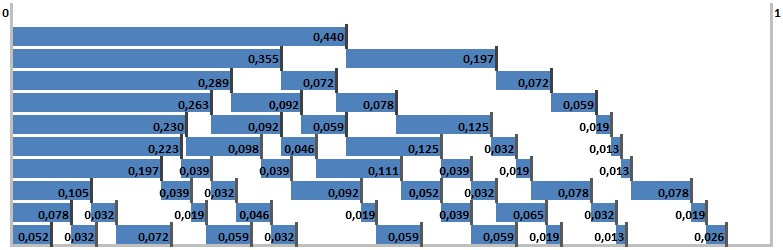
\includegraphics[scale=.7]{sections/images/consciousness_logical_moments.jpg}
	\floatfoot{Exemplo de um intervalo lógico com dez momentos lógicos.}%\footnotemark}
	\end{figure}
	%\footnotetext{Fonte: note}

A consciência são os momentos lógicos de uma expansão representados em suas unidades.
	\begin{figure}[H]
	\caption{Intervalo lógico consciente}
	\label{fig:consciousness}
	\centering
	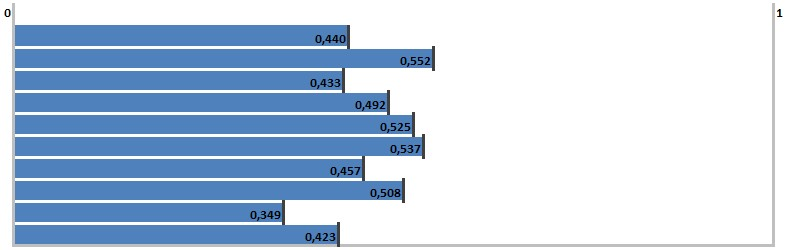
\includegraphics[scale=.7]{sections/images/consciousness.jpg}
	\floatfoot{Exemplo de um intervalo lógico consciente com dez unidades de momentos lógicos.}%\footnotemark}
	\end{figure}
	%\footnotetext{Fonte: note}

Pode ser observado na Tabela \ref{tab:10000_all} que a probabilidade de 99,99\% das amostras (Amostras do Range), que aumentam em quantidade a medida que crescem os momentos lógicos, tendem a estar cada vez mais ao centro do intervalo lógico, sendo que essa centralização tende ao infinito.
	\begin{figure}[H]
	\caption{Centralização de 99,99\% das amostras}
	\label{fig:centering_of_99_range}
	\centering
	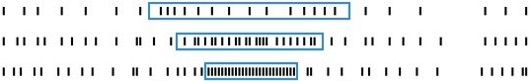
\includegraphics[scale=1]{sections/images/centering_of_99_range.jpg}
	\floatfoot{Tendência de centralização do range de 99,99\% das amostras.}%\footnotemark}
	\end{figure}
	%\footnotetext{Fonte: note}

A consciência tende à representação de um histograma da distribuição normal. Todos os aspectos listados abaixo são inerentes a abstração lógica chamada consciência.

\subsubsection{Infinito}
Um dos aspectos mais importantes que a negação do nada traz (negação de si), é o infinito, ou seja, em qualquer intervalo lógico cabe o infinito novamente. A lógica primordial que iniciou todo o intervalo lógico é a mesma encontrada em seus intervalos subsequentes. Isso fundamenta como uma lógica de alto nível como a subconsciência humana explica a lógica primordial, uma vez que não é preciso voltar ao primeiro momento lógico do intervalo para deduzi-lo, pois esse fenômeno é onipresente em todo o intervalo.

\subsubsection{Ondas}
Probabilisticamente a distribuição de novas amostras de uma população tendem a concentrar mais amostras sentido a mediana da população com frequências de amostras cada vez maiores neste sentido. Porém, a distribuição dessas amostras com frequências de crescimento uniformes é infinitesimal se comparado às possibilidades randômicas desse crescimento. Assim, a tendência de crescimento dessas frequências sentido a mediana somadas a baixíssima probabilidade (infinitesimal) desse crescimento ser uniforme, conduz a frequências no padrão de ondas.
	\begin{figure}[H]
	\caption{Padrão de onda}
	\label{fig:consciousness_waves}
	\centering
	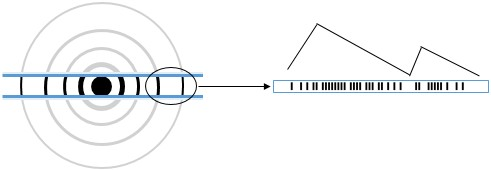
\includegraphics[scale=1]{sections/images/consciousness_waves.jpg}
	\floatfoot{Padrão de onda inferido pela tendência dessa distribuição com frequências maiores sentido a mediana da população e a baixíssima probabilidade de crescimento uniforme dessas frequências.}%\footnotemark}
	\end{figure}
	%\footnotetext{Fonte: note}

A junção de duas ondas além de eliminar suas discrepâncias, faz com que a primeira onda da união fique maior e a segunda onda acabe por deixar de existir a se tornar parte da primeira, que tem seu pico mais próximo da mediana. Probabilisticamente uma onda não morre, apenas une-se com outras ondas mais centrais a ela.
	\begin{figure}[H]
	\caption{Unificação de ondas}
	\label{fig:consciousness_uniform_wave}
	\centering
	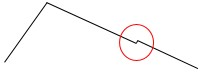
\includegraphics[scale=1]{sections/images/consciousness_uniform_wave.jpg}
	\floatfoot{Ondas sendo unificadas para exemplificar o crescimento amostral uniforme.}%\footnotemark}
	\end{figure}
	%\footnotetext{Fonte: note}

\subsubsubsection{Entrelaçamento e subconsciente}
As amostras que mais se parecem em termos de frequências e distribuição são as amostras que fazem parte da mesma onda. Elas são frequências opostas não sobrepostas que se completam.

Probabilisticamente as duas partes complementares de uma onda estarão a uma distância aproximadamente iguais, equidistante da mediana, porém essa não é uma regra e as partes complementares de uma onda podem estar em distâncias diferentes da mediana. O fenômeno da paridade das partes de uma onda tem o nome de entrelaçamento de ondas.

Essas ondas formam subconsciências de uma consciência maior. A consciência é única para todo o intervalo, é a lógica do intervalo, enquanto formam subconsciências, como pequenas ondas de uma onda maior. Assim, uma mudança na onda maior (consciência) também é uma mudança na onda menor (subconsciência), mudança essa que é induzida pelas subconsciências indiretamente, análogo ao comprimir gás em um cilindro, onde ao adicionar uma nova molécula de gás no cilindro parcialmente cheio, mais próximas ou apertas as moléculas dentro dele estarão. O contrário também é verdadeiro, uma nova amostra em uma subconsciência que por esta é observada diretamente é também uma mudança da consciência e vai ser induzida por outras subconsciências indiretamente.
	\begin{figure}[H]
	\caption{Subconsciência}
	\label{fig:consciousness_subconscious}
	\centering
	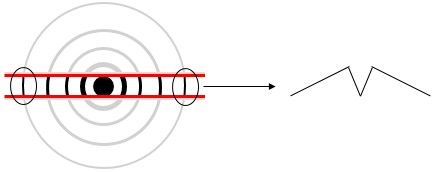
\includegraphics[scale=1]{sections/images/consciousness_subconscious.jpg}
	\floatfoot{O padrão de ondas forma subconsciências semelhantes ao padrão criado pela consciência (histograma de distribuição normal) como visto na Figura \ref{fig:statisticsbyjim_central_limit_theorem} ou na Figura \ref{fig:trend_chart_of_normal_distribution}.}%\footnotemark}
	\end{figure}
	%\footnotetext{Fonte: note}

\subsubsubsection{Salto}
O salto é uma reordenação feita pelo entrelaçamento de ondas a medida que as amostras do entrelaçamento deixam de ser equivalentes com a adição de novas amostras em seus lados.

Na Figura \ref{fig:consciousness_space_subconscious_observation_jump} é observado os entrelaçamento de ondas (representadas por colunas do histograma na vertical). A reordenação feita pelo entrelaçamento provoca um salto nas coordenadas (X, Y e Z) conforme subseção do Espaço.
	\begin{figure}[H]
	\caption{Reordenação subconsciente - Salto}
	\label{fig:consciousness_space_subconscious_observation_jump}
	\centering
	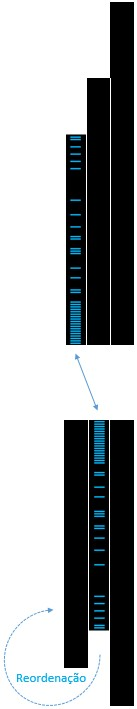
\includegraphics[scale=.6]{sections/images/consciousness_space_subconscious_observation_jump.jpg}
	\floatfoot{Salto provocado pela não equivalência do entrelaçamento com a adição de novas amostras.}%\footnotemark}
	\end{figure}
	%\footnotetext{Fonte: note}

A tendência probabilística é que, por exemplo, o elétron que saltou de sua orbita de origem retorne à esta conforme mais amostras são adicionadas ao entrelaçamento desse átomo, estabelecendo a normalidade probabilística.

\subsubsection{Tempo}
O tempo é a adição de novos momento lógicos entre momentos existentes à medida que prossegue a negação de si da lógica. Essas mudanças são acumulativas e a medida que aumentam o número desses momentos lógicos, menos relevante cada novo momento será dentro do intervalo consciente. Um em cem é mais relevante do que um em mil. 
	\begin{figure}[H]
	\caption{Tempo}
	\label{fig:consciousness_time}
	\centering
	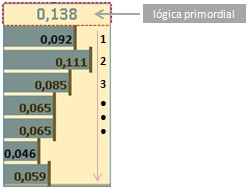
\includegraphics[scale=.8]{sections/images/consciousness_time.jpg}
	\floatfoot{Progressão do tempo conforme os momentos lógicos avançam.}%\footnotemark}
	\end{figure}
	%\footnotetext{Fonte: note}

Outro fator importante a observar do tempo é que, probabilisticamente, subconsciências mais próximas da mediana da população terão uma adição maior de novas amostras em seus intervalos, o que são observados diretamente por essas subconsciências. Por outro lado, subconsciências distantes da mediana da população terão uma adição menor de amostras em seus intervalos e sujeitam-se a um número maior de mudança induzidas indiretamente. Esse fenômeno de observação temporal proporcionado pela consciência e subconsciências evita o paradoxo dos gêmeos \cite{brasilescola_paradoxo_gemeos}.

Na seção Expansão lógica foi apresentado que a lógica é uma sequência de negações de si no tempo zero, ou seja, em nenhum momento entre suas negações a lógica passa a SER, garantindo a premissa primordial da constante lógica, NÃO SER. Assim, a lógica é uma sequência infinita e simultânea, uma constante. Logo, o tempo é apenas uma grandeza da consciência oriunda da ordenação dessa sequência lógica, não da sequência propriamente. A simultaneidade dessa sequência torna a lógica uma constante com todas as suas infinitas possibilidades, sendo esse universo uma delas. 

Cada universo tem uma ordem diferente em sua sequência e é essa ordem que dá origem à grandeza que chamamos de tempo. É essa ordem do universo ou consciência que vai dar a noção do que acontece antes ou depois, ou seja, o passado, o presente e o futuro. 

Na experiência do tempo conduzida pela consciência a ordenação da sequência é a essência dessa grandeza e, portanto, mais relevante do que sua origem que é de natureza simultânea.

\subsubsection{Espaço}
As ondas da consciência exibidas em forma de histograma, onde as partes das ondas que se completam são colocados lado a lodo é exibida na Figura \ref{fig:consciousness_space_waves}. A formação desse histograma é proveniente do entrelaçamento de ondas.
	\begin{figure}[H]
	\caption{Histograma proveniente do entrelaçamento de ondas}
	\label{fig:consciousness_space_waves}
	\centering
	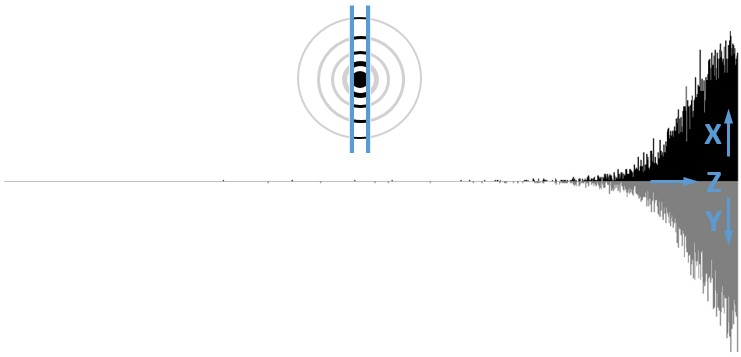
\includegraphics[scale=.7]{sections/images/consciousness_space_waves.jpg}
	\floatfoot{Exemplo do padrão de ondas obtido pelo algoritmo Logic\_WavePattern. \footnotemark}
	\end{figure}
	\footnotetext{O algoritmo Logic\_WavePattern pode ser visto no Apêndice \ref{app:algoritmos}.}

Ao representar as grandezas espaciais do gráfico da Figura \ref{fig:consciousness_space_waves} em um gráfico de distribuição 3D e distribuir seus pontos de extremidade (desprezando seus volumes e possíveis pontos internos), obtém-se algo parecido com uma espiral (como redemoinhos no ar ou na água) mesmo em volumes muito pequenos de dados (poucos momentos lógicos), conforme Figuras \ref{fig:consciousness_space_3DScatter15000-10} e \ref{fig:consciousness_space_3DScatter_200000-2}. Os pontos se movem em formato de espiral, aproximadamente, uma vez que as coordenadas X, Y e Z aumentam à medida que novas amostras são adicionadas na população.
	\begin{figure}[H]
	\centering
		\begin{subfigure}[H]{0.47\linewidth}
		\centering
		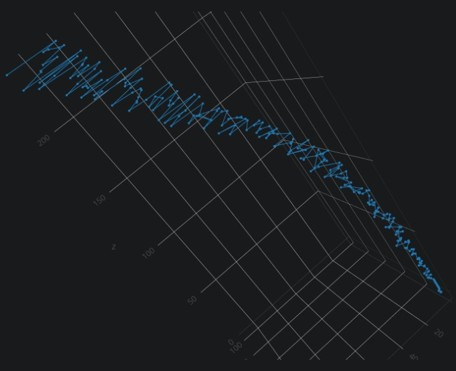
\includegraphics[width=.96\linewidth]{sections/images/consciousness_space_3DScatter15000-10.jpg}
		\caption{15.000 amostras ou momentos}
		\label{fig:consciousness_space_3DScatter15000-10}
		\end{subfigure}
	\hfill
		\begin{subfigure}[H]{0.47\linewidth}
		\centering
		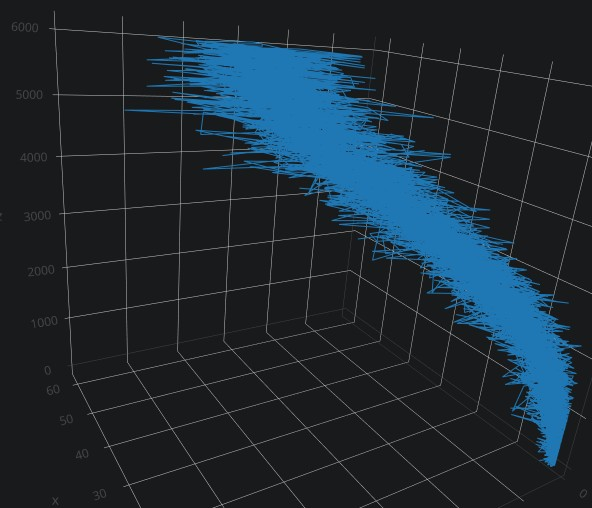
\includegraphics[width=.9\linewidth]{sections/images/consciousness_space_3DScatter_200000-2.jpg}
		\caption{200.000 amostras ou momentos}
		\label{fig:consciousness_space_3DScatter_200000-2}
		\end{subfigure}%
	\caption{Gráfico de dispersão 3D gerado com os pontos da Figura \ref{fig:consciousness_space_waves}}
	\floatfoot{O histograma no padrão de ondas e os dados para gerar o gráfico de dispersão 3D podem ser obtidos com a execução do algoritimo Logic\_WavePattern. \protect\footnotemark}
	\end{figure}
	\footnotetext{O algoritmo Logic\_WavePattern pode ser visto no Apêndice \ref{app:algoritmos} e os gráficos de dispersão 3D podem ser acessados em: \url{https://chart-studio.plot.ly/create/?fid=ren.stuchi:5&fid=ren.stuchi:4} e \url{https://chart-studio.plot.ly/create/?fid=ren.stuchi:7&fid=ren.stuchi:6}}

\subsubsubsection{Intervalos}
A observação de outras subconsciências depende do range de ondas que uma subconsciência é capaz de observar e esse range, por sua vez depende do range de ondas que a própria subconsciência é constituída. Todos os possíveis intervalos que se correspondem em X e Y encontram-se simultaneamente formando ondas em diferentes níveis.

Em ranges de muitos momentos lógicos pode-se ver o agrupamento de grandes objetos (subconsciências), sendo o maior deles representado pela cor azul claro e os menores e mais distantes pela cor azul escuro ou roxo, conforme Figura \ref{fig:consciousness_space_subconsciousness}. Esse agrupamento pode representar, por exemplo, o centro do universo, então o centro de uma galáxia, estrelas, planetas e objetos menores e mais distantes.
	\begin{figure}[H]
	\caption{Abstração espacial das subconsciências - grandes agrupamentos}
	\label{fig:consciousness_space_subconsciousness}
	\centering
	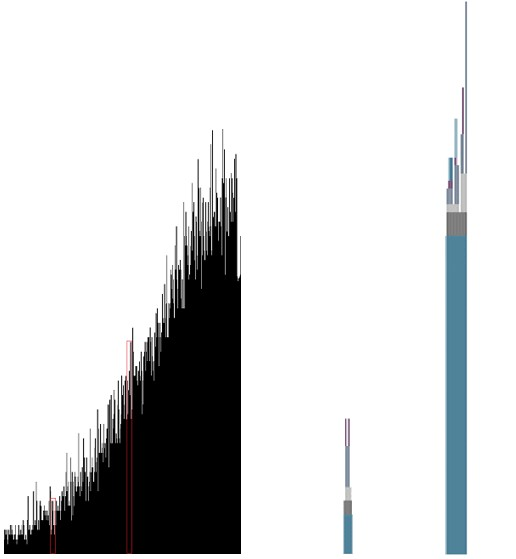
\includegraphics[scale=.5]{sections/images/consciousness_space_subconsciousness.jpg}
	\floatfoot{Caracteristicas da ondas formadoras da subconsciência de grandes objetos.}%\footnotemark}
	\end{figure}
	%\footnotetext{Fonte: note}

Em ranges com uma quantidade menor de momentos lógicos pode-se ver o agrupamento de pequenos objetos (subconsciências). Quanto menores os agrupamentos menos divisões esses agrupamentos têm (cores) e mais estreitos e compridos eles são, conforme Figura \ref{fig:consciousness_space_subconsciousness_min}. Esse agrupamento pode representar, por exemplo, o átomo que são muito pequenos, se apresentam em enormes quantidades e as partículas que orbitam seu núcleo (elétrons) ficam bem mais distantes dele.
	\begin{figure}[H]
	\caption{Abstração espacial das subconsciências - pequenos agrupamentos}
	\label{fig:consciousness_space_subconsciousness_min}
	\centering
	
\includegraphics[scale=.7]{sections/images/consciousness_space_subconsciousness_min.jpg}
	\floatfoot{Caracteristicas da ondas formadoras da subconsciência de pequenas partículas.}%\footnotemark}
	\end{figure}
	%\footnotetext{Fonte: note}}
	
As cores dos agrupamentos indicam a relação entre conjuntos e subconjuntos. Subconjuntos nascem de conjuntos ou outros subconjuntos e essa relação paterna filial é permanente. Conjuntos e subconjuntos também podem se dividir no mesmo nível, a depender do entrelaçamento das amostras.

\subsubsubsection{Volume}
O volume dobra a cada um terço de crescimento das amostras ou momentos lógicos de um agrupamento, aproximadamente. Como exibido na Figura \ref{fig:consciousness_space_volume}, os momentos lógicos ficam mais concentrados no começo das ondas entrelaçadas, o que pode gerar algo de fácil observação nessa região, como estrelas, planetas etc. 
\begin{figure}[H]
	\caption{Amostras vs volume}
	\label{fig:consciousness_space_volume}
	\centering
	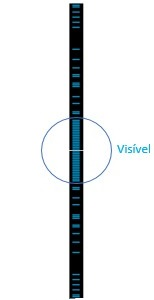
\includegraphics[scale=.8]{sections/images/consciousness_dark_matter_dark_energy_wave.jpg}
	\floatfoot{O volume em três dimensões dobra a cada um terço de crescimento das amostras, aproximadamente.}%\footnotemark}
	\end{figure}
	%\footnotetext{Fonte: note}}

\subsubsubsection{Espiral}
Os subconjuntos de um agrupamento tendem a formar espirais em seus movimentos que podem ser melhor entendidas e observadas na Figura \ref{fig:consciousness_space_spiral}.

Cada agrupamento tem sua própria linha de referência. Assim como dentro de um metro existem os centímetros, milímetros etc., dentro de um agrupamento existem outros agrupamentos.
	\begin{figure}[H]
	\caption{Detalhes do movimento em espiral}
	\label{fig:consciousness_space_spiral}
	\centering
	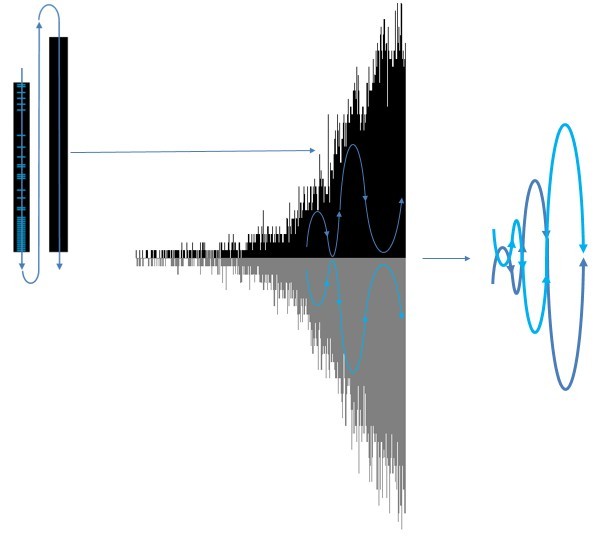
\includegraphics[scale=.8]{sections/images/consciousness_space_spiral.jpg}
	\floatfoot{Detalhes do movimento em espiral dos subconjuntos de amostras.}%\footnotemark}
	\end{figure}
	%\footnotetext{Fonte: note}}

Na Figura \ref{fig:consciousness_space_spiral} foi refletida as amostras da linha de referência para os eixos X e Z para facilitar as observações. As observações abaixo relacionadas ao eixo X também se aplicam ao eixo Y:
	\begin{description}
	   \item[Linha de referência] Representa uma diagonal entre os eixos X, Y e Z onde os subconjuntos (traços como representados no exemplo de A e B) estão dispostos ao redor dessa linha e se afastando dela à medida que os valores das coordenadas aumentam.
	   \item[A e B] Os traços representados no exemplo de A e B são subconjuntos de uma população. Quando mais amostras em um subconjunto mais estável e harmônicos são seus movimentos espirais probabilísticos em torno de sua linha de referência. Os subconjuntos em A representam a média mínima probabilística de X para esse intervalo Z. Já os subconjuntos em B representam a média máxima probabilística de X para esse intervalo Z. Visto que os subconjuntos se dispõem probabilisticamente ao redor da linha de referência, então os subconjuntos e A por estarem na média mínima tendem probabilisticamente a receber mais amostras que os subconjuntos em B, fazendo com que os subconjuntos em A se elevem em X mais rapidamente que os subconjuntos em B que por estarem recebendo menos amostras, nesse cenário, passam a estar em uma elevação de X menor.
	   \item[X1 e X2] A adição de novas amostras à população formam novos subconjuntos antes e depois dos representados por A e B. Assim, as coordenadas X, Y e Z de A e B aumentam e faz com que esses se movimentem a frente, como exemplificado por B. É importante notar que os subconjuntos em B mesmo com uma elevação probabilística em X menor continuam a aumentar o valor de X mesmo com a impressão de que o valor X diminuiu, conforme mostrado por X1 e X2.
	\end{description}

Na Figura \ref{fig:consciousness_space_spiral_direction} é exibida a orientação da parte visível de um objeto juntamente com o espaço que completa a formação deste objeto.
	\begin{figure}[H]
	\caption{Orientação do movimento em espiral}
	\label{fig:consciousness_space_spiral_direction}
	\centering
	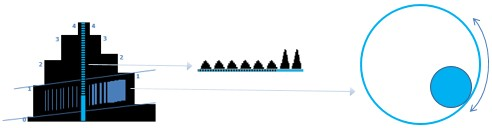
\includegraphics[scale=1]{sections/images/consciousness_space_spiral_direction.jpg}
	\floatfoot{Detalhes do orientação do movimento em espiral dos subconjuntos de amostras.}%\footnotemark}
	\end{figure}
	%\footnotetext{Fonte: note}}
	
\subsubsection{Forças fundamentais}
A força gravitacional, a força eletromagnética e a força nuclear correspondem às forças fundamentais da natureza e essas forças também são provenientes do entrelaçamento de ondas, como o espaço. As forças fundamentais não são forças propriamente, mas sim aspectos probabilísticos (distribuição normal) e do entrelaçamento de ondas principalmente.

\subsubsubsection{Força gravitacional}
O entrelaçamento ondas é o aspecto que coordena as mudanças nas coordenadas espaciais junto com a adição de novos momentos lógicos sentido a mediana da população. As mudanças dessas coordenadas provocam iterações que podem ser vistas nas Figuras \ref{fig:consciousness_space_3DScatter15000-10} e \ref{fig:consciousness_space_3DScatter_200000-2} da subseção de Espaço e na Figura \ref{fig:consciousness_dark_matter_dark_energy_wave} que mostra probabilisticamente onde está a maior concentração de momentos lógicos de um intervalo consciente ou subconsciente, devido a estes momentos serem mais intensos sentido a mediana. Estes aspectos são chamadas de gravidade.

\subsubsubsection{Força eletromagnética}
A força eletromagnética é uma especificação do aspecto gravitacional que depende da aproximação espacial (redução de diferenças nos eixos X, Y e Z) e do entrelaçamento de ondas.

Quando um objeto se aproxima de outro, seus pares de ondas provenientes do entrelaçamento de ondas ficam cada vez mais parecidos, eixos X e Y. Essa proximidade faz com que as partes das ondas de um objeto se pareça muito com as partes das ondas do outro objeto, o que pode fazer com que o entrelaçamento de ondas encontre pares mais ideais nesse outro objeto e vice-versa.  

As linhas azuis da Figura \ref{fig:consciousness_electromaagnetic_force} mostra onde é mais frequente a troca dos pares de ondas pelo entrelaçamento de ondas, ou seja, onde se tem a maior probabilidade das ondas serem parecidas. Por isso os imãs tentam se virar para se conectar quando estão face a face com o mesmo polo. As linhas cinza mostram as conexões que ocorrem em número bem menor. 
	\begin{figure}[H]
	\caption{Força eletromagnética}
	\label{fig:consciousness_electromaagnetic_force}
	\centering
	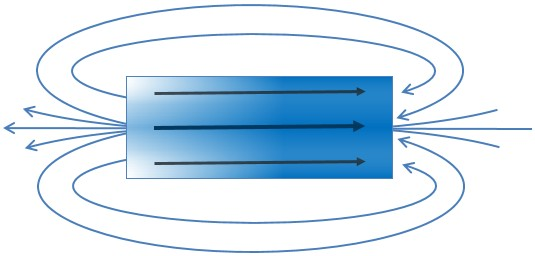
\includegraphics[scale=.6]{sections/images/consciousness_electromaagnetic_force.jpg}
	\floatfoot{Aumento das possibilidades de entrelaçamento de ondas devida a aproximação e o menor número de momentos lógicos das menores partículas. }%\footnotemark}
	\end{figure}
	%\footnotetext{Fonte: note}

Com a troca de significativos pares de ondas entre os objetos faz-se a mixagem do posicionamento dos eixos X, Y e Z entre esses objetos ocorrendo a aproximação deles no espaço. 

Quanto menor a partícula (elétron ou partículas menores), conforme Figura \ref{fig:consciousness_space_subconsciousness_min}, mais fácil o entrelaçamento ocorre. Provavelmente muitos objetos não tenham alta capacidade de entrelaçamento devido aos seus elétrons ou partículas menores serem formadas por muitos momentos lógicos (barras do histograma mais largas ou mais compridas), ou seja, quanto maior a quantidade de momentos dessas partículas menores as chances de entrelaçamento.

Probabilisticamente as partículas mais parecidas estão nas regiões mais próximas (linhas azuis do Figura \ref{fig:consciousness_electromaagnetic_force}) devido ao crescimento do número de amostras sentido a mediana da população, porém isso não é uma regra e os polos podem se inverter, ou seja, ter mais ligações com a região de menor probabilidade (isso não quer dizer que houve formação de antimatéria nessa região, as partículas ainda tendem a concentrar mais momentos lógicos sentido à mediana da população). No entanto, a probabilidade tende a corrigir esses polos conforme novos momentos vão sendo adicionadas nesse intervalo.

\subsubsubsection{força nuclear}
As forças nucleares forte e fraca representam as maiores concentrações de momentos lógicos por intervalo populacional. Esses picos podem ser vistos na Figura \ref{fig:consciousness_space_subconsciousness_min} e eles não param de crescer à medida que novos momentos lógicos são adicionados nestes intervalos. Estes momentos ou amostras tendem a estarem cada vez mais juntos dentro do intervalo formando picos cada vez mais altos.

\subsubsection{Matéria escura e energia escura}
Quanto maior o número de amostras e mais próximas elas estão da mediana, mais elas farão parte dos 99,99\% e ainda mais amostras também estarão nos 0,01\%, conforme a Tabela \ref{tab:10000_all}. Logo, a energia escura não é uma energia propriamente, mas sim um aspecto probabilístico. 
	\begin{figure}[H]
	\caption{Aspecto probabilístico da energia escura}
	\label{fig:consciousness_dark_matter_dark_energy}
	\centering
	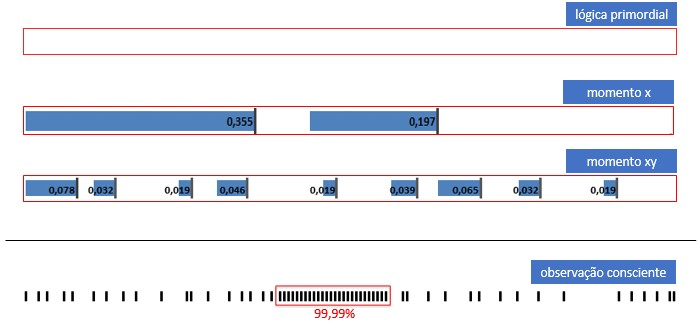
\includegraphics[scale=1]{sections/images/consciousness_dark_matter_dark_energy.jpg}
	\floatfoot{A energia escura não é uma energia propriamente, mas sim um aspecto probabilístico.}%\footnotemark}
	\end{figure}
	%\footnotetext{Fonte: note}

Já a matéria escura, como pode ser visto na Figura \ref{fig:consciousness_dark_matter_dark_energy_wave} mostra probabilisticamente onde está a maior concentração das amostras de um intervalo, tornando mais fácil a visualização por outras subconsciências, uma vez também que o volume dobra a cada um terço do crescimento das colunas do histograma, aproximadamente, conforme dito na seção do Espaço. Assim, uma grande área do intervalo de um agrupamento pode conter amostras dispersas que se tornam mais difíceis de observar. O aspecto descrito acima e demostrado pela Figura \ref{fig:consciousness_dark_matter_dark_energy_wave} é aplicável a qualquer intervalo de um agrupamento (Figuras \ref{fig:consciousness_space_subconsciousness} e \ref{fig:consciousness_space_subconsciousness_min}).
	\begin{figure}[H]
	\caption{Analogia da matéria escura}
	\label{fig:consciousness_dark_matter_dark_energy_wave}
	\centering
	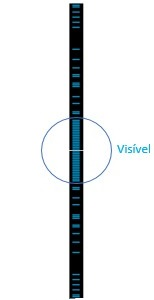
\includegraphics[scale=.9]{sections/images/consciousness_dark_matter_dark_energy_wave.jpg}
	\floatfoot{Parte do volume é facilmente observado por outras subconsciências.}%\footnotemark}
	\end{figure}
	%\footnotetext{Fonte: note}

\subsubsection{Antimatéria}
Independente do intervalo observado, sua maior concentração de amostras tende a estar sentido da mediana, o que é o sentido provável conforme teorema central do limite. Essas amostras também podem estar com sua concentração no sentido oposto à mediana, porém com uma ocorrência probabilística cada vez menos conforme as amostras aumentam. Na Figura \ref{fig:consciousness_concentration_of_opposite_samples} é exibido dois intervalos idênticos com suas amostras com concentrações opostas.
	\begin{figure}[H]
	\caption{Parte de um intervalo idêntico com suas concentrações de amostras opostas}
	\label{fig:consciousness_concentration_of_opposite_samples}
	\centering
	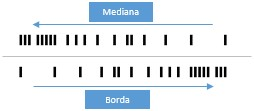
\includegraphics[scale=1]{sections/images/consciousness_concentration_of_opposite_samples.jpg}
	\floatfoot{Parte de um intervalo idêntico distribuídos de formas opostas.}%\footnotemark}
	\end{figure}
	%\footnotetext{Fonte: note}

O merge ou soma dos intervalos opostos da Figura \ref{fig:consciousness_concentration_of_opposite_samples} os tornaria um intervalo simétrico, ou seja, não estaria em nenhum dos sentidos.
Na Figura \ref{fig:consciousness_concentration_of_opposite_samples_within_range} é exibido um intervalo consciente completo com suas concentrações de amostras sentido à mediana e outro idêntico, mas com suas concentrações sentido às bordas do intervalo.
	\begin{figure}[H]
	\caption{Intervalos conscientes com suas concentrações de amostras opostas}
	\label{fig:consciousness_concentration_of_opposite_samples_within_range}
	\centering
	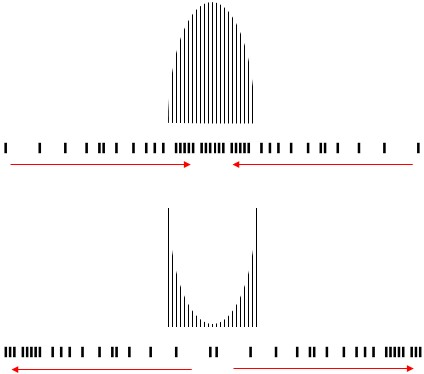
\includegraphics[scale=.8]{sections/images/consciousness_concentration_of_opposite_samples_within_range.jpg}
	\floatfoot{Intervalos conscientes completos e idênticos distribuídos de formas opostas.}%\footnotemark}
	\end{figure}
	%\footnotetext{Fonte: note}


\subsubsection{Buraco negro}
O buraco negro é uma concentração muito alta de amostras, formada por grandes agrupamentos subconscientes, Figura \ref{fig:consciousness_space_subconsciousness}.
Esses grandes agrupamentos ocupam grandes volumes de espaço devido a quantidade de amostras. 

Os grandes volumes são encontrados na base dos grandes agrupamentos, conforme as cores azul claro e cinza da Figura \ref{fig:consciousness_black_hole}.
	\begin{figure}[H]
	\caption{Buracos negros}
	\label{fig:consciousness_black_hole}
	\centering
	
\includegraphics[scale=.6]{sections/images/consciousness_black_hole.jpg}
	\floatfoot{Grandes volumes são encontrados na base dos grandes agrupamentos.}%\footnotemark}
	\end{figure}
	%\footnotetext{Fonte: note}

% ----------------------------------------------------------
% Subseção Observações
% ----------------------------------------------------------
\subsection{Observações}

\begin{description}
   \item[Rigidez lógica] Se a rigidez física e suas leis parecem ser intransponíveis, abaixo dela está à lógica, ainda mais rígida e intransponível, pois fora da lógica o que se tem é o inexistente, o ilógico. A existência está contida nas possibilidades do que é lógico. 
   \item[Matemática] A matemática é uma ótima abstração do universo, mas ela não é a linguagem do universo, pois abaixo da matemática está à lógica, a base da matemática e de toda a existência.
   \item[Bem e mal] O bem e o mal são observações das subconsciências. Ou seja, se está claro a negação tende a escurecer, se está calor a esfriar etc. É a briga dos contrários de Heráclito de Éfeso.
   \item[Perfeição] A lógica primordial é a mais simples das lógicas, é a essência da existência. Uma lógica tão simples quanto eficiente, tão eficiente quanto perfeita. A lógica mais poderosa:
   \begin{description}
	   \item[Onipotente] A essência de todas as possibilidades lógicas, ou seja, a essência da existência, pois fora das possibilidades lógicas está o ilógico, o inexistente;
	   \item[Onisciente] Fluxo de todas as abstrações lógicas desde a consciência às subconsciências; 
	   \item[Onipresente] Suas frações (negações) estão em toda a existência.
   \end{description}
Essas observações remetem a Deus, a consciência das subconsciências.
   \item[Realidade] Como possibilidade lógica o sonho é tão real quando a "realidade". Talvez o estudo das possibilidades lógicas leve a caminhos onde os sonhos possam ser tão reais quanto à realidade, já que os dois não passam de lógica, como sonhos lúcidos, por exemplo \cite{ administradores_principio_pareto}. Isso talvez explique por que outras possíveis formas de vidas "inteligentes", quando evoluídas, deixam de buscar esse tipo de vida em um possível vasto universo à procurarem dentro de si, onde se pode encontrar algo bem maior que o universo, o infinito.
\end{description}
		
		% Finaliza a parte no bookmark do PDF, para que se inicie o bookmark na raiz
		\bookmarksetup{startatroot}% 
		
		% Conclusão
		% ----------------------------------------------------------
% Considerações Finais
% ----------------------------------------------------------
\section*{Considerações Finais}
\addcontentsline{toc}{section}{Considerações finais}
Este é um estudo da lógica primordial que resultou em uma teoria a respeito da origem de tudo. Todas as linhas de raciocínio deste estudo podem ser aprofundadas e detalhadas. 

Eventualmente pode ser considerado um estudo filosófico e/ou científico, entretanto a base desses dois importantes ramos é a lógica, o núcleo dessa teoria. 

A resposta da pergunta central desse estudo (se existe algo ao invés de nada) vem da lógica. O estudo da lógica deu origem a uma teoria a respeito da origem de todas as coisas. Essa teoria reponde o que é a consciência, as ondas, o infinito, o tempo, o espaço, as forças fundamentais, a matéria escura, a energia escura, a antimatéria, o buraco negro e o observador e a vida.

Que o modelo desse estudo seja o início de uma nova era. Uma era onde o ser humano possa desenvolver a si e observar que é o hospedeiro do infinito. Que essa evolução possa transformar os sonhos em realidade e que seja possível observar que a realidade não é diferente de um sonho, uma vez que ambas são apenas lógicas.

Pensar que algo físico tenha surgido do nada se faz incoerente com a natureza do nada.


	% ----------------------------------------------------------
	% ELEMENTOS PÓS-TEXTUAIS
	% ----------------------------------------------------------
	\postextual
		
		% Referências bibliográficas
		\bibliography{sections/references}{}
		
		% Apêndices
		% ----------------------------------------------------------
% APÊNDICE A - Algorithms
% ----------------------------------------------------------
\begin{apendicesenv}
\chapter{Algorithms}
\label{app:algorithms}
\subsection*{BinomialDistribution\_PROB and Distribution\_PROB}
%\enlargethispage{40mm}
The BinomialDistribution\_PROB algorithm generates the probability of distribution of an interval and uses the general binomial probability formula below. This algorithm has the same result as the Distribution\_PROB algorithm, but the BinomialDistribution\_PROB execution is much faster and has higher capacity because it uses large numbers like BigInteger and BigDecimal. Both algorithms were done in C\# with LINQPad 5 \footnotemark. The Figure \ref{fig:BinomialDistribution_PROB_and_Distribution_PROB} shows the results of the algorithms for the range 0 to 10, analogous to flipping 10 coins on the ground, adding up the values of the heads and tails, with the tails having the value one and the heads having the value two. The Distribution\_PROB algorithm sums each of the 1024 possibilities [1,1,1,1,1,1,1,1,1,1,1,1 - 1,1,1,1,1,1,1,1,1,1,1, 2 - ....] and groups these values together. In the Distribution\_PROB algorithm, this set of possibilities is a Cartesian product of the possible combinations, which makes this algorithm slow, but it is important to validate and facilitate understanding of the general binomial probability formula used in the BinomialDistribution\_PROB algorithm \cite{mathisfun_binomial_distribution}. In the Figure \ref{fig:BinomialDistribution_PROB_and_Distribution_PROB}, the table within Distribution\_PROB shows this grouping and the total number of possibilities, 1024. Dividing each grouped value by the total gives the probabilistic result achieved by the formula used in BinomialDistribution\_PROB. For example, the probability that the sum of the 10 coins flipped is 12 is equal to 45/1024, or 0.0439453125 or 4.39\%.
\footnotetext{LINQPad 5 is on \url{www.linqpad.net} and can be used in its free version (Standard edition) without expiration.}
%\enlargethispage{-50mm}
	\begin{align*}
	f(k;n,p) &= \binom{n}{k} p^k(1 - p)^{n-k}
	\end{align*}
	\begin{figure}[H]
	\caption{Results of the BinomialDistribution\_PROB and Distribution\_PROB algorithms}
	\label{fig:BinomialDistribution_PROB_and_Distribution_PROB}
	\centering
	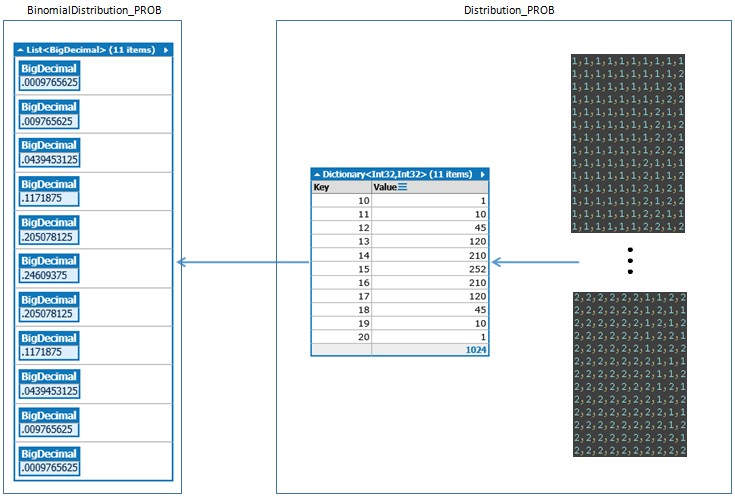
\includegraphics[scale=.77]{sections/images/BinomialDistribution_PROB_and_Distribution_PROB.jpg}
	\floatfoot{The Distribution\_PROB algorithm intends to clarify the probabilistic essence of the central limit theorem.} %\footnotemark.
	\end{figure}

The Distribution\_PROB algorithm can also be used for the roll of 5 6-sided dice or 6 5-sided dice, for example. As can be seen in the Figure below, the probability distribution on the dice roll is similar to the binomial distribution (coins).
	\begin{figure}[H]
	\centering
		\begin{subfigure}[H]{0.47\linewidth}
		\centering
		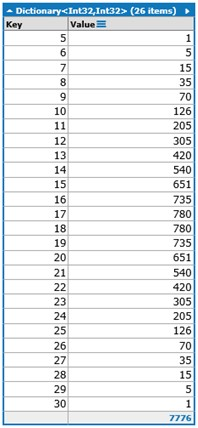
\includegraphics[width=.6\linewidth]{sections/images/Distribution_PROB_5_6.jpg}
		\caption{5 6-sided dice}
		\label{fig:Distribution_PROB_5_6}
		\end{subfigure}
	\hfill
		\begin{subfigure}[H]{0.47\linewidth}
		\centering
		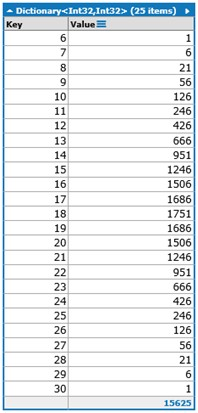
\includegraphics[width=.62\linewidth]{sections/images/Distribution_PROB_6_5.jpg}
		\caption{6 5-sided dice}
		\label{fig:Distribution_PROB_6_5}
		\end{subfigure}%
	\caption{Results of the Distribution\_PROB algorithm}
	\floatfoot{The probability distribution on the dice roll is consonant to the binomial distribution.} %\protect\footnotemark
	\end{figure}

\subsubsection*{BinomialDistribution\_PROB [Code]}
To execute the code snippet requires the implementation of BigDecimal, an example of that implementation can be seen, obeying proprietary software license rights, at \cite{github_bigdecimal}. This study does not distribute nor is it responsible for the portion of the code related to the BigDecimal implementation, these responsibilities being the responsibility of the executor of this software.

\bigbreak
\begin{lstlisting}
//https://www.mathsisfun.com/data/quincunx-explained.html
void Main()
{
    BinomailDistribuition.Possibilities = 10;
    var results = new List<BigDecimal>();
    results.Load();
    results.Print(true); //send false to print Table 1.
}

public static class BinomailDistribuition
{
    public static int Possibilities = 0;
    static int middleLeft = 0;
    static int middleRight = 0;
    static int resultCount = 0;
    
    public static void Load(this List<BigDecimal> results)
    {
        for (int i = 0; i <= Possibilities; i++)
        {
            var fatorLeft = Fatorial(Possibilities);
            var fatorRight = BigInteger.Multiply(Fatorial(i), Fatorial(Possibilities - i));
            BigInteger fat = BigInteger.Divide(fatorLeft, fatorRight);
            var powLeft = new BigDecimal(1, 0, 1000000000);
            var powRight = new BigDecimal(1, 0, 1000000000);
            if (i != 0)
                powLeft = BigDecimal.Pow(new BigDecimal(5, 1, 1000000000), i);
            if (i != Possibilities)
                powRight = BigDecimal.Pow(new BigDecimal(5, 1, 1000000000), (Possibilities - i));
            var prob = new BigDecimal(fat) * powLeft * powRight;
            results.Add(prob);
        }
    }
    
    public static BigInteger Fatorial(int value)
    {
        BigInteger fatorial = 1;
        for (int n = 1; n <= value; n++)
        {
            fatorial *= n;
        }
        return fatorial;
    }
    
    public static void Print(this List<BigDecimal> results, bool printTableProbability)
    {
        if (!printTableProbability)
        {
            var sum = results.Sum();
            var middle = (middleRight - middleLeft) / 2;
            var middlePercent = ((middleRight - middleLeft) * 14) / 100;
            var list = results.Where((x, i) => i >= middleLeft && i <= middleRight).ToList();
            var listPareto = list.Where((x, i) => i >= (middle - middlePercent) 
                                               && i <= (middle + middlePercent)).ToList();
            var percentOfSum = (middleRight - middleLeft) * 100 / resultCount;
            var sumPercent = sum * new BigDecimal(100, 0, 1000000000);
            var paretoResult = new BigDecimal(0, 0, 1000000000);
            listPareto.ForEach(x => { paretoResult = paretoResult + x; });

            sumPercent.Dump("sum");
            middleLeft.Dump("middleLeft");
            middleRight.Dump("middleRight");
            (middleRight - middleLeft).Dump("itens of sum");
            percentOfSum.Dump("percent of sum");
            resultCount.Dump("total");
            paretoResult.Dump("20/80");
        }
        else
        {
            results.Dump(); //Valid Binomial distribution    
        }
    }
    
    public static BigDecimal Sum(this List<BigDecimal> results)
    {
        resultCount = results.Count;
        middleLeft = resultCount / 2;
        middleRight = middleLeft * 2 < resultCount ? middleLeft + 1 : middleLeft;

        var sum = middleLeft != middleRight ? results[middleLeft] + results[middleRight] : results[middleRight];
        while ((sum * new BigDecimal(100, 0, 1000000000)) < new BigDecimal(9999, 2, 1000000000))
        {
            middleLeft--;
            middleRight++;
            if (middleLeft >= 0)
                sum = sum + results[middleLeft];
            if (middleRight <= Possibilities)
                sum = sum + results[middleRight];
        }
        return sum;
    }
}

//Exemple of BigDecimal class - https://github.com/dparker1/BigDecimal/blob/
//3e0a4f1ba4c72c0b28d6571fcc6259558be104bd/BigDecimal/BigDecimal.cs
\end{lstlisting}

\bigbreak
\bigbreak
\subsubsection*{Distribution\_PROB [Code]}
\begin{lstlisting}
//https://exercicios.brasilescola.uol.com.br/exercicios-matematica/
//exercicios-sobre-probabilidade-condicional.htm#questao-1
void Main()
{
    var dice = 2; //Binomial distribution, dice = 2;
    var events = 10;
    var sampling = Math.Pow(dice, events);
    var cartesianProduct = dice.ToArrays(events).CartesianProduct();
    cartesianProduct.PrintGroup(events, dice);
}

public static class CartesianProductContainer
{
    public static IEnumerable<IEnumerable<int>> CartesianProduct(this IEnumerable<IEnumerable<int>> sequences)
    {
        IEnumerable<IEnumerable<int>> emptyProduct = new[] { Enumerable.Empty<int>() };
        var result = sequences.Aggregate(
            emptyProduct,
            (accumulator, sequence) =>
                from accseq in accumulator
                from item in sequence
                select new[] { accseq.Concat(new[] { item }).Sum() });

        return result;
    }

    public static IEnumerable<List<int>> ToArrays(this int dice, int events)
    {
        var result = new List<List<int>>();
        for (int j = 1; j <= events; j++)
        {
            var array = new List<int>();
            for (int i = 1; i <= dice; i++)
                array.Add(i);
            
            result.Add(array);
        }

        return result;
    }
    
    public static void PrintGroup(this IEnumerable<IEnumerable<int>> list, int events, int dice)
    {
        var listCountDict = Enumerable.Range(1, dice * events).ToDictionary(x => x);
        Group(listCountDict, list);
        listCountDict.Dump("Values");
    }

    public static void Group(Dictionary<int, int> dict, IEnumerable<IEnumerable<int>> list)
    {
        foreach (var key in dict.Keys.ToList())
            dict[key] = 0;

        foreach (var item in list)
            dict[item.First()]++;

        var zeroKey = 0;
        foreach (var item in dict)
            if (item.Value == 0) 
                zeroKey = item.Key;
            else continue;

        for (int i = 1; i <= zeroKey; i++)
            dict.Remove(i);
    }
}

\end{lstlisting}


\bigbreak \bigbreak
\subsection*{Logic\_WavePattern}
The Logic\_WavePattern algorithm results in the display of a histogram that assumes the wave pattern when placed side by side each of the bars on the left and right side of the median. This histogram is generated from randomizing the values according to Figure \ref{fig:consciousness_logical_moments} and Figure \ref{fig:consciousness}, following the central limit theorem.
	\begin{figure}[H]
	\caption{Histogram in the wave pattern of the Logic\_WavePattern algorithm}
	\label{fig:logic_wavepattern_15000}
	\centering
	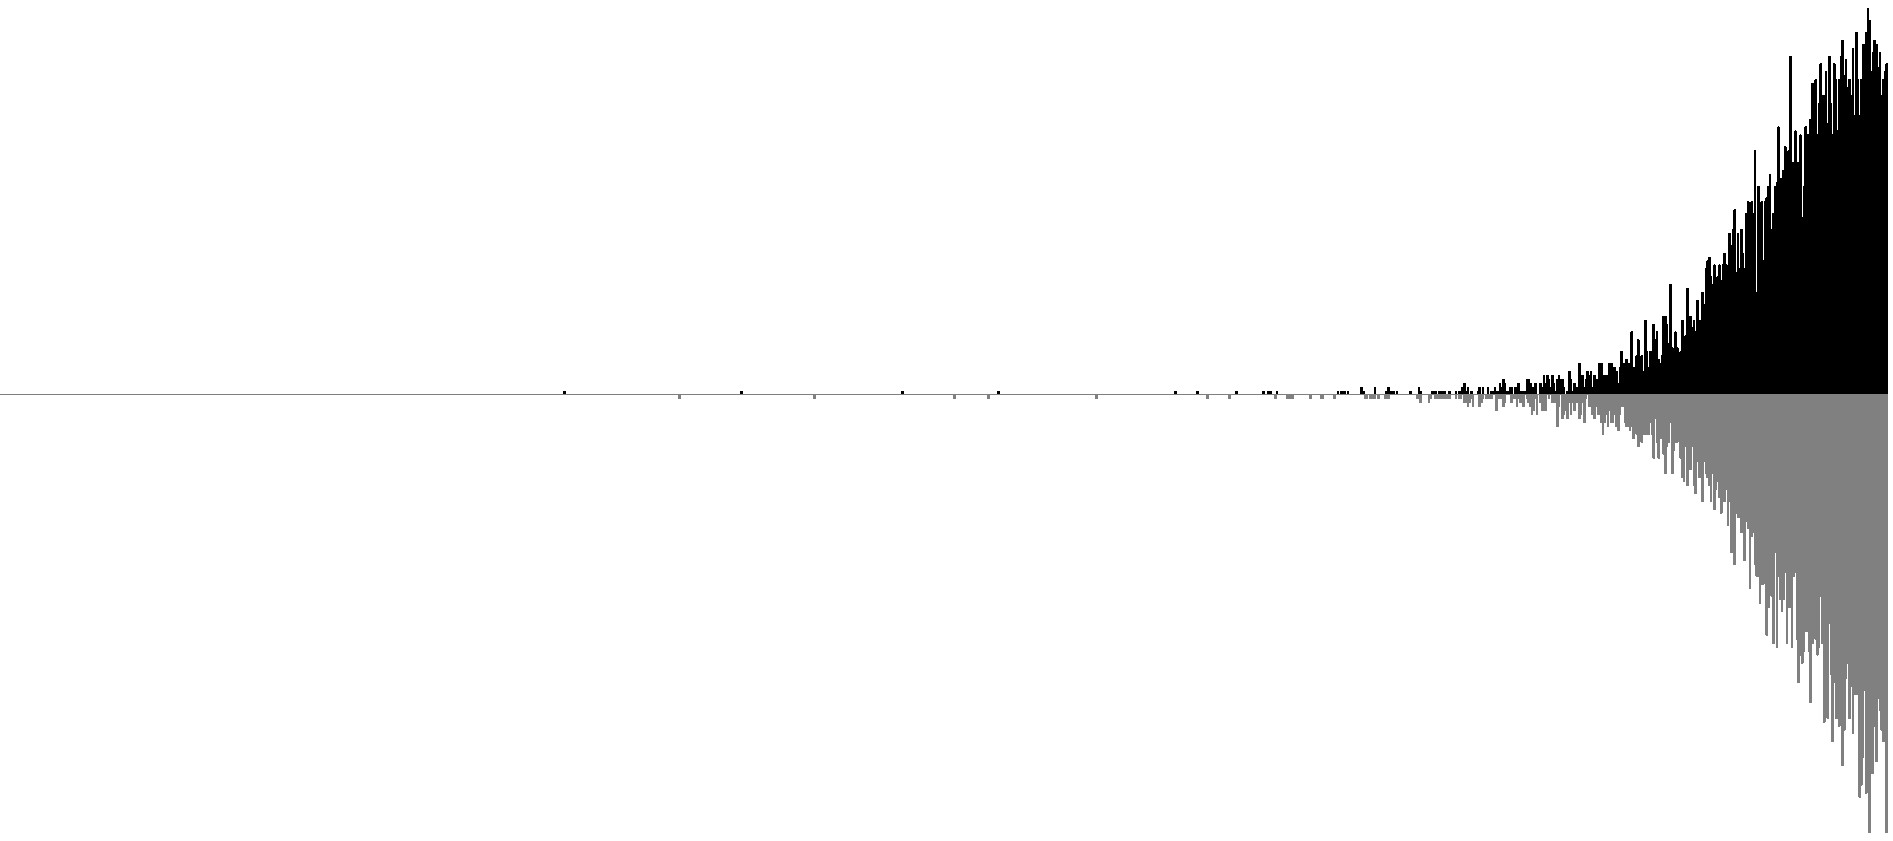
\includegraphics[scale=.25]{sections/images/logic_wavepattern_15000.jpg}
	\floatfoot{Randomly generated result displayed by the Logic\_WavePattern algorithm.} %\footnotemark.
	\end{figure}

Another result of the Logic\_WavePattern algorithm is obtained from the LINQPad 5 console, which outputs a file in ".csv" format that can be imported into Plotly's Chart Studio \url{https://chart-studio. plot.ly/create} for generating a 3D scatter plot. The most important part of the graph are the points that represent the most easily visible part and that are most likely at the top of each histogram bar in the previous Figure. Lines are used to facilitate the visualization of spirals that are already starting to form even with very low volumes of data and without the entanglement of intervals (ordering).
	\begin{figure}[H]
	\caption{3D scatter plot of the Logic\_WavePattern algorithm}
	\label{fig:plotly_3DScatter}
	\centering
	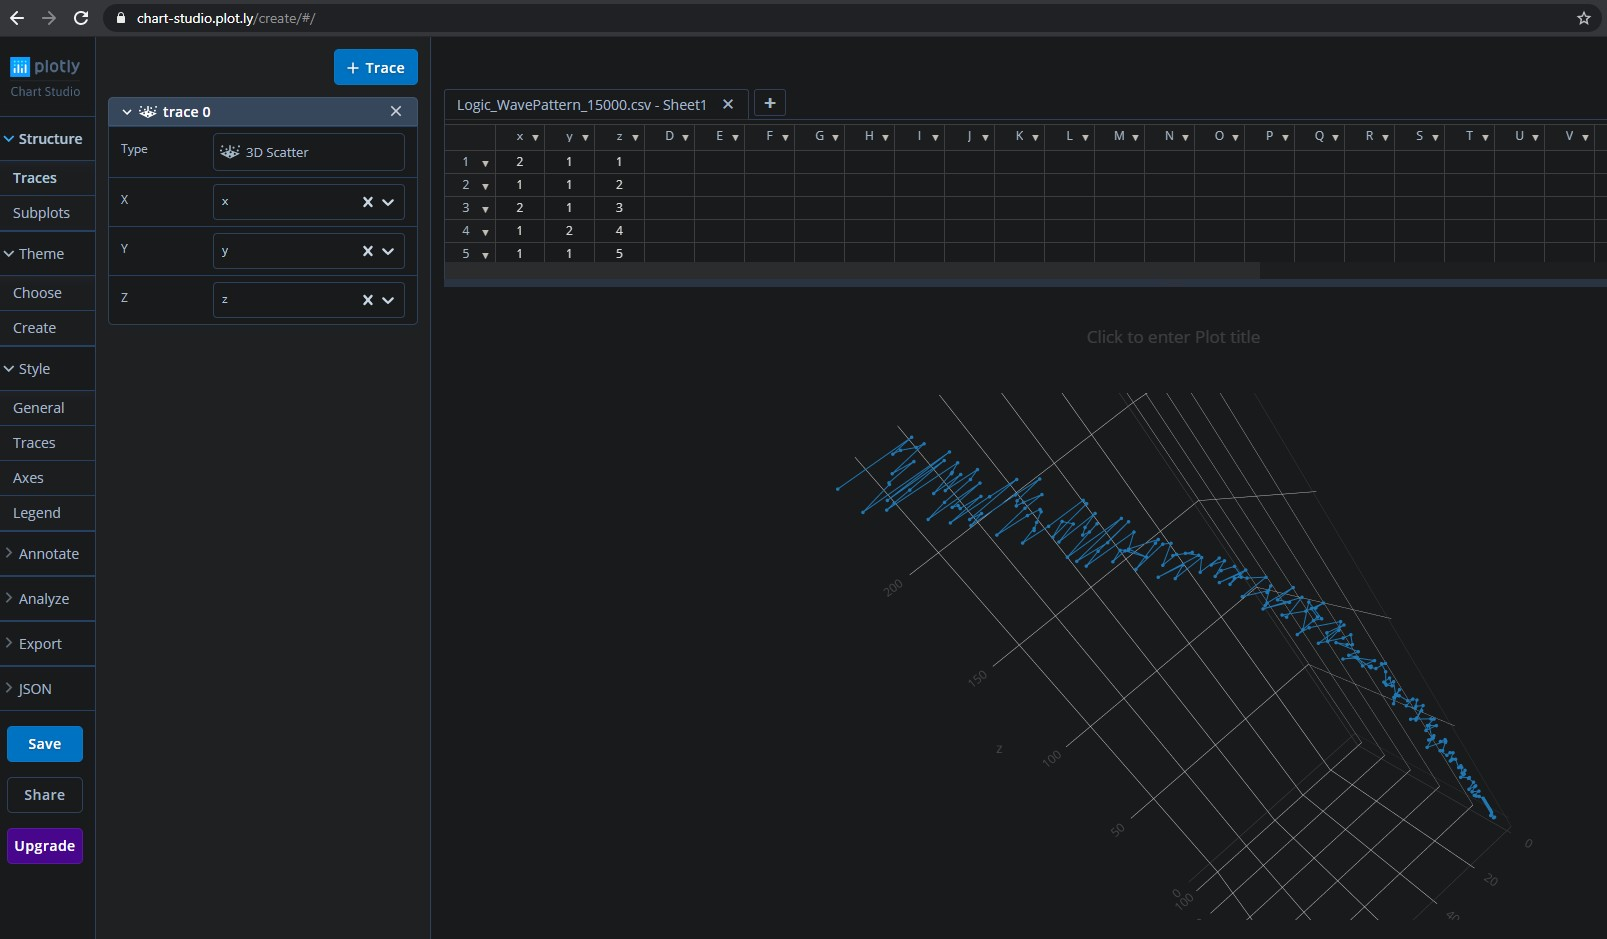
\includegraphics[scale=.33]{sections/images/plotly_3DScatter.jpg}
	\floatfoot{The example can be accessed at: \url{https://chart-studio.plot.ly/create/?fid=ren.stuchi:5&fid=ren.stuchi:4}.} %\footnotemark.
	\end{figure}

\subsubsection*{Logic\_WavePattern [Code]}
\begin{lstlisting}
//http://csharphelper.com/blog/2015/09/draw-a-simple-histogram-in-c/
//https://github.com/naudio/NAudio.WaveFormRenderer
[STAThread]
void Main()
{
  Application.EnableVisualStyles();
  Application.Run(new MainForm());
}

public partial class MainForm : Form
{
  public MainForm()
  {
    InitializeComponent();
  }
  //###########################################################################
  private const int LENGHT = 30000;
  private const int GROUP = 2;
  //###########################################################################
  private double m_dZoomscale = 1.0;
  public static double s_dScrollValue = .25;
  private Point MouseDownLocation;
  private Matrix transform = null;
  private NumbsOfCentralLimitTheorem.HistogramResult histogramResult = null;
  private bool printed = false;

  private void MainForm_Load(object sender, EventArgs e)
  {
    histogramResult = GetHistogramOfCentralLimitTheorem(LENGHT, GROUP);

    RectangleF data_bounds = new RectangleF(0, 0, histogramResult.Size, histogramResult.MaxValue * 2);
    PointF[] points =
    {
        new PointF(0, pictHistogram.ClientSize.Height),
        new PointF(pictHistogram.ClientSize.Width, pictHistogram.ClientSize.Height),
        new PointF(0, 0)
      };
    transform = new Matrix(data_bounds, points);
  }

  private void pictHistogram_Paint(object sender, PaintEventArgs e)
  {
    DrawHistogram(e.Graphics, pictHistogram.BackColor, histogramResult,
      pictHistogram.ClientSize.Width, pictHistogram.ClientSize.Height);
  }

  private void pictHistogram_Resize(object sender, EventArgs e)
  {
    pictHistogram.Refresh();
  }

  private void DrawHistogram(Graphics gr, Color back_color,
    NumbsOfCentralLimitTheorem.HistogramResult histogramResult, int width, int height)
  {
    PrintResult();
    gr.Clear(back_color);
    gr.Transform = transform;
    gr.ScaleTransform((float)m_dZoomscale, (float)m_dZoomscale);
    FillRectangle(gr, Color.Black, histogramResult.Up, histogramResult.MaxValue, false);
    FillRectangle(gr, Color.Gray, histogramResult.Down, histogramResult.MaxValue, true);
  }

  private void PrintResult()
  {
    if (!printed)
    {
      printed = true;
      var listTuple = new List<(float x, float y, float z)>();
      float previousValueOfZ = 0;
      for (int i = 0; i < histogramResult.Up.Count(); i++)
      {
        if (histogramResult.Up[i] != 0.0001f && histogramResult.Down[i] != 0.0001f)
        {
          if (histogramResult.Up[i] % 1 == 0)
            previousValueOfZ = (int)(previousValueOfZ + 1f);
          else
            previousValueOfZ += 0.1f;
          var tuple = (x: histogramResult.Up[i], y: histogramResult.Down[i], z: previousValueOfZ);
          listTuple.Add(tuple);
        }
      }
      Console.WriteLine("x,y,z");
      foreach (var tuple in listTuple)
        Console.WriteLine(tuple.x.ToString() + "," + tuple.y.ToString() + "," + tuple.z.ToString());
    }
  }

  protected void FillRectangle(Graphics gr, Color color, float[] arrayValues, float maxValue, bool down)
  {
    using (Pen thin_pen = new Pen(color, 0))
    {
      for (int i = 0; i < histogramResult.Down.Length; i++)
      {
        RectangleF rect;
        if (!down)
          rect = new RectangleF(i, maxValue, 1, arrayValues[i]);
        else
          rect = new RectangleF(i, maxValue - arrayValues[i], 1, arrayValues[i]);
        using (Brush the_brush = new SolidBrush(color))
        {
          gr.FillRectangle(the_brush, rect);
          gr.DrawRectangle(thin_pen, rect.X, rect.Y, rect.Width, rect.Height);
        }
      }
    }
  }

  protected void pictHistogram_OnMouseWheel(object sender, MouseEventArgs mea)
  {
    pictHistogram.Focus();
    if (pictHistogram.Focused == true && mea.Delta != 0)
      ZoomScroll(mea.Location, mea.Delta > 0);
  }

  private void ZoomScroll(Point location, bool zoomIn)
  {
    transform.Translate(-location.X, -location.Y);
    if (zoomIn)
      m_dZoomscale = m_dZoomscale + s_dScrollValue;
    else
      m_dZoomscale = m_dZoomscale - s_dScrollValue;
    transform.Translate(location.X, location.Y);
    pictHistogram.Invalidate();
  }

  private void pictHistogram_MouseDown(object sender, MouseEventArgs e)
  {
    if (e.Button == System.Windows.Forms.MouseButtons.Left)
      MouseDownLocation = e.Location;
  }

  private void pictHistogram_MouseMove(object sender, MouseEventArgs e)
  {
    if (e.Button == System.Windows.Forms.MouseButtons.Left)
    {
      transform.Translate((e.Location.X - MouseDownLocation.X)
        / 40, (e.Location.Y - MouseDownLocation.Y) / 40, MatrixOrder.Append);
      this.Refresh();
    }
  }

  private NumbsOfCentralLimitTheorem.HistogramResult GetHistogramOfCentralLimitTheorem(int length, int group)
  {
    var numbsOfCentralLimitTheorem = new NumbsOfCentralLimitTheorem();
    numbsOfCentralLimitTheorem.RandomResult(length);
    return numbsOfCentralLimitTheorem.GenerateHistogram(group);
  }
}

partial class MainForm
{
  private System.ComponentModel.IContainer components = null;

  protected override void Dispose(bool disposing)
  {
    if (disposing && (components != null))
      components.Dispose();
    base.Dispose(disposing);
  }

  private void InitializeComponent()
  {
    this.pictHistogram = new System.Windows.Forms.PictureBox();
    ((System.ComponentModel.ISupportInitialize)(this.pictHistogram)).BeginInit();
    this.SuspendLayout();
    this.pictHistogram.Anchor = ((System.Windows.Forms.AnchorStyles)((((System.Windows.Forms.AnchorStyles.Top
          | System.Windows.Forms.AnchorStyles.Bottom)
          | System.Windows.Forms.AnchorStyles.Left)
          | System.Windows.Forms.AnchorStyles.Right)));
    this.pictHistogram.BackColor = System.Drawing.Color.White;
    this.pictHistogram.Cursor = System.Windows.Forms.Cursors.Cross;
    this.pictHistogram.Location = new System.Drawing.Point(8, 6);
    this.pictHistogram.Name = "pictHistogram";
    this.pictHistogram.Size = new System.Drawing.Size(550, 250);
    this.pictHistogram.TabIndex = 1;
    this.pictHistogram.TabStop = false;
    this.pictHistogram.Resize += new System.EventHandler(this.pictHistogram_Resize);
    this.pictHistogram.Paint += new System.Windows.Forms.PaintEventHandler(this.pictHistogram_Paint);
    this.pictHistogram.MouseWheel += new System.Windows.Forms.MouseEventHandler(this.pictHistogram_OnMouseWheel);
    this.pictHistogram.MouseDown += new System.Windows.Forms.MouseEventHandler(this.pictHistogram_MouseDown);
    this.pictHistogram.MouseMove += new System.Windows.Forms.MouseEventHandler(this.pictHistogram_MouseMove);
    this.AutoScaleDimensions = new System.Drawing.SizeF(6F, 13F);
    this.AutoScaleMode = System.Windows.Forms.AutoScaleMode.Font;
    this.ClientSize = new System.Drawing.Size(563, 262);
    this.Controls.Add(this.pictHistogram);
    this.Name = "MainForm";
    this.Text = "Logic_WavePattern";
    this.Load += new System.EventHandler(this.MainForm_Load);
    ((System.ComponentModel.ISupportInitialize)(this.pictHistogram)).EndInit();
    this.ResumeLayout(false);
  }

  internal System.Windows.Forms.PictureBox pictHistogram;
}

public class NumbsOfCentralLimitTheorem
{
  public float[] ResultList { get; set; }
  public int ResultLength { get; set; }
  public float[] LastList { get; set; }
  public float[] CurrentList { get; set; }
  public int SizeLastList { get; set; }
  public Dictionary<int, float> Histogram { get; set; }

  public NumbsOfCentralLimitTheorem()
  {
    SizeLastList = 2;
    StartLastList();
    StartCurrentList();
  }

  public float[] RandomResult(int length)
  {
    ResultLength = length;
    ResultList = new float[length];
    Random rnd = new Random();
    for (int x = 0; x < length; x++)
    {
      float lineSum = 0;
      for (int i = 1; i < SizeLastList; i++)
      {
        var lastValueLeft = LastList[i - 1];
        var lastValueRight = LastList[i];
        var rndValue = (float)rnd.NextDouble(lastValueLeft, lastValueRight);
        lineSum = lineSum + (rndValue - lastValueLeft);
        CurrentList[i] = rndValue;
      }
      if (lineSum != 0)
        ResultList[x] = lineSum;
      SizeLastList++;
      LastList = CurrentList;
      StartCurrentList();
    }
    return ResultList;
  }

  public HistogramResult GenerateHistogram(int group)
  {
    Histogram = new Dictionary<int, float>();
    var minValue = ResultList.Min();
    var maxValue = ResultList.Max();
    var rangeValue = maxValue - minValue;
    var amountOfGroups = ResultLength / group;
    var intervalValue = rangeValue / amountOfGroups;
    foreach (var value in ResultList)
    {
      int key = (int)(value / intervalValue);
      if (!Histogram.ContainsKey(key))
        Histogram[key] = 0;
      Histogram[key]++;
    }
    var histogramResult = HistogramResult.Get(Histogram);
    return histogramResult;
  }

  private void StartCurrentList()
  {
    var sizeCurrentList = SizeLastList + 1;
    CurrentList = new float[sizeCurrentList];
    CurrentList[0] = 0;
    CurrentList[sizeCurrentList - 1] = float.MaxValue / 2; 
  }

  private void StartLastList()
  {
    LastList = new float[SizeLastList];
    LastList[0] = 0;
    LastList[SizeLastList - 1] = float.MaxValue / 2; 
  }

  public class HistogramResult
  {
    public int Size { get; set; }
    public float MaxValue { get; set; }
    public float[] Up { get; set; }
    public float[] Down { get; set; }

    public static HistogramResult Get(Dictionary<int, float> histogram)
    {
      var histogramOrdered = histogram.OrderBy(k => k.Key);
      var result = new HistogramResult();
      var lengthOdd = histogram.Count % 2 > 0;
      var middle = histogram.Count / 2;
      var middleValue = histogramOrdered.ElementAt(middle).Key;
      result.Size = middleValue;
      result.MaxValue = histogram.OrderBy(k => k.Value).Last().Value;
      result.Up = ArrangeArray(new float[middleValue]);
      result.Down = ArrangeArray(new float[middleValue]);
      for (int i = 0; i < middle; i++)
      {
        var keyValue = histogramOrdered.ElementAt(i);
        result.Up[keyValue.Key] = keyValue.Value;
      }
      for (int i = lengthOdd ? middle + 2 : middle + 1; i < histogram.Count; i++)
      {
        var totalValue = middleValue * 2;
        var keyValue = histogramOrdered.ElementAt(i);
        result.Down[totalValue - keyValue.Key] = keyValue.Value;
      }
      return result;
    }

    private static float[] ArrangeArray(float[] array)
    {
      for (int i = 0; i < array.Length; i++)
        array[i] = 0.0001F;
      return array;
    }
  }
}

public static class rndExtension
{
  public static double NextDouble(this Random rng, double minimum, double maximum)
  {
    return rng.NextDouble() * (maximum - minimum) + minimum;
  }
}
\end{lstlisting}

\end{apendicesenv}

\end{document}